\documentclass[11pt]{article}

\usepackage{common}
\usepackage{float}
\usepackage{pythonhighlight}
\usepackage{booktabs}

%This changes removes indentation and instead adds space between paragraphs. I think it looks nicer this way. 
\setlength{\parindent}{0pt}
\setlength{\parskip}{0.5ex}

\title{\textbf{CS181 Practical}}
\author{\textbf{Ty Geri, Elias Nuwara, Ben Ray} \\ tygeri@college.harvard.edu\\
eliasab@college.harvard.edu\\
benray@college.harvard.edu}
\date{\textbf{April/May 2022}}

\begin{document}

\maketitle{}

\section{Part A: Feature Engineering, Baseline Models}

\subsection{Approach}
PCA is a method of dimensionality reduction. In summary, it takes the features from the audio clips (our data) and reduces these features into a lower-dimensional basis. It chooses this lower dimensional basis by selecting the eigenvectors corresponding to the largest eigenvalues of the empirical covariance matrix (calculated from the centered data). These eigenvectors are the principal components of the data, which correspond to the directions of largest variance in the features from the audio clips.\\

\noindent We calculate 500 principal components using the training data and use these (the top 500 directions of largest variance in the data) to construct the lower-dimensional representation of our features, using \texttt{PCA.fit\_transform(X\_train)}.\\

\noindent Logistic regression is a supervised probabilistic classification method. This means that we will start with the functional form of a generalized linear model ($\boldy = \boldw^\top \boldx$), convert this to a conditional distribution ($p(\boldy=C_k | \boldx) = \text{softmax}_k(\boldw^\top \boldx)$), and then optimize the weights and parameters of the conditional distribution directly using a maximum likelihood procedure such as gradient descent. The logistic regression classifier ultimately assigns a data point to a class according to which $C_k$ maximizes $p(\boldy=C_k | \boldx)$.\\

\noindent Having first used PCA to reduce the dimensionality of our data, we fit the logistic regression model using the "saga" solver with L2 regularization, using \texttt{LogisticRegression.fit(X\_train\_pca, y\_train)}.

\subsection{Results}
The results for the PCA \& logistic regression models can be found in section 3.1. The overall training accuracy, overall test accuracy, and per-class classification accuracy can be found in \textit{Table 1}. The actual per-class classification results can be seen in the two confusion matrices \textit{AMP: PCA \& Logistic Regression Confusion Matrix} and \textit{MEL: PCA \& Logistic Regression Confusion Matrix}.\\

\subsection{Discussion}

The model trained on MEL data outperformed the model trained on AMP data on all metrics shown in Table 1 (overall training accuracy, overall test accuracy, and per-class classification accuracy). This mainly resulted from the MEL-trained model doing a much better job of predicting rare classes such as class 1 and 6, for which the AMP-trained model could not predict any sounds correctly. In addition, both classifiers seem to disproportionately predict class 2, potentially because this - ``children playing" - can easily be mistaken for other sounds.\\

\noindent The reason for the disparity in performance between the two models is likely due to the way that the data was generated. The AMP data is effectively the raw sound data, while the MEL data is generated using a short-time Fourier transform. Thus, the MEL data is a lot less noisy: the Fourier transformation captures the signal of the sound modelled by a summation of sine and cosine functions, rather than capturing every detail of the noise included in the AMP data.\\

\noindent We use PCA to reduce overfitting to very noisy training data (especially for AMP data). Thus, our test accuracy ended up being higher when we first used PCA to reduce the dimensionality of our data. Furthermore, it is a waste of computational power to fit the logistic regression model to redundant components of the data that only capture the noise (e.g. background noise, echoes, etc.) in the recorded sound. Thus, we chose to fit the model to only the top 500 principal components that capture the most variance between the different sounds, i.e. the most useful ones for classification.

\section{Part B: More Modeling}

\subsection{Part B1: Random Forests}

\subsubsection{Approach}
We chose to use a random forest model as our classifier. Random forests are a large collection of decision trees that together create an ensemble. Effectively, we take the most frequent prediction from the decision trees in order to maximize our predictive accuracy. Since the trees are uncorrelated with each other, as a collective, they should give insight into more likely classifications.\\ 

\noindent Decision trees themselves work by figuring out how to best split the data into recursively smaller datasets in order to make our classification prediction. The max depth of the tree indicates the number of splits we can make.\\

\noindent In general random forests work as such:
\footnote{\text{https://dataaspirant.com/random-forest-algorithm-machine-learing/\#:~:text=Random%20Forest%20pseudocode%3A&text=Among%20the%20%E2%80%9Ck%E2%80%9D%20features%2C,%E2%80%9Cn%E2%80%9D%20number%20of%20trees.
}}
\begin{enumerate}
    \item Randomly choose i features from m total features
    \item Place the best feature (within the i features) as the root node (the best split point)
    \item Split the node into child nodes again using the best split point
    \item Repeat 1 - 3 until max depth
    \item Repeat to create n decision trees
    \item Predict using the test data the classifications for all decision trees
    \item Take the classification with the highest frequency among the n decision trees
\end{enumerate}

\noindent In practice, we used \texttt{RandomForestClassifier} from \texttt{scikit-learn}:

\begin{python}
from sklearn.ensemble import RandomForestClassifier

# RandomForest
model = RandomForestClassifier(n_estimators=500, max_depth=32, n_jobs=-1)
model.fit(X_mel_train_flat.reshape(X_mel_train_flat.shape[0], -1), y_mel_train)

# Make our predictions
rf_preds = model.predict(X_mel_test_flat.reshape(X_mel_test_flat.shape[0], -1))
print(np.mean(rf_preds == y_mel_test))
\end{python}

\subsubsection{Results}
The results for the random forest models can be found in section 3.2. The overall training accuracy, overall test accuracy, and per-class classification accuracy can be found in \textit{Table 2}. The actual per-class classification results can be seen in the two confusion matrices \textit{AMP: Random Forest Confusion Matrix} and \textit{MEL: Random Forest Confusion Matrix}.

\subsubsection{Discussion}
Like with our PCA \& logistic regression models, the random forest trained on MEL data outperformed the one trained on AMP data on all metrics shown in Table 2 (overall training accuracy, overall test accuracy, and per-class classification accuracy). This again resulted from the MEL-trained model doing a much better job of predicting rare classes such as class 1 and 6, for which the AMP-trained model could not predict any sounds correctly. In addition, with the random forests, the AMP-trained model disproportionately predicted class 2 significantly more than the MEL-trained model, as can be seen by looking at the confusion matrices.\\

\noindent As we can see from comparing \textit{Table 1} and \textit{Table 2}, the random forest models performed much better than the PCA \& logistic regression models. Logistic regression models work well when the data is linearly separable. This is rare, however, in the real world. Since the logistic regression classifier fails to predict AMP and MEL data with reasonable accuracy, we can assume that the datasets are not linearly separable. From that assumption we began to brainstorm which models would work best for non-linearly separable data. We considered using a convolutional neural network but ran into some issues since CNNs are more often used for visual classification than audio classification. Instead, we opted for random forests, an ensemble version of a decision tree model. Decision tree models are prone to overfitting the data but by using many trees, as we do in the random forest, we can generalize our model better.\\ 

\noindent Yet, even with our random forest running at max-depth our model failed to get significant improvement on the AMP data. This leads us to a conclusion that the AMP data is simply too noisy, as we can't, even with overfitting-prone max-depth, predict it with reasonable probability.\\ 

\noindent We can see from Table 2 that our training accuracy is 100\%. This is a clear sign of overfitting and is a result of using decision trees of too great a depth. However, we came to using decision trees of depth 32 after running our cross-validation and testing various different depths and number of trees. The outcome, discussed in more detail below, was that we achieved optimal test predictability with a depth of 32. Therefore, we left it as 32. We tested trees of depths 4, 8, and 16 and found much lower training accuracy as in line with the theory, but proceeded with 32 in order to maximize our overall test accuracy.\\ 

\noindent In terms of improvements on the test accuracy:
\begin{center}
    AMP-trained models improved by $34\%$ from the logistic regression model to the random forest\\ 
    MEL-trained models improved by $44\%$ from the logistic regression model to the random forest
\end{center}
While the test accuracies of the random forest are still not very high (i.e. none scoring above 50\% accuracy), these improvements are significant and show the power of non-linear classifiers in real-world situations.

\subsection{Part B2: Hyperparameter Tuning and Validation}

\subsubsection{Approach}
It's not an easy task to find the optimal hyperparameters for an ML model. The choice of hyperparamters could lead to underfitting or overfitting the training data.\\

\noindent When we performed the model training discussed above, we used the training dataset that was provided to us for training and the separate testing dataset for testing (although the selection of datasets to use for each is usually done randomly). It is worth noting that a problem with this approach of splitting the entire data just once into training and testing is that we may end up leaving out some important observations from the model training.\\

\noindent We would usually try to solve this problem with cross-validation. Cross-validation reduces the likelihood of missing out on some important information in the data by randomly splitting the data into training and validation sets and repeating multiple times. We applied this concept to tune the hyperparameters for both our PCA \& logistic regression and  random forest models, using 5-fold cross-validation.\\

\noindent For the PCA \& logistic regression models, we decided to tune the parameter \texttt{C} - the strength of L2 regularization (effectively the coefficient $\lambda$ that we have used for regularization in CS181). We tested 5 different hyperparameter values, $[0.25, 0.5, 1, 1.5, 2]$ - values selected around the \texttt{scikit-learn} default of $1$ and ran tuning with cross-validation on these values using the \texttt{GridSearchCV} function.\\

\noindent For the random forest model, we decided to tune two different hyperparameters: the maximum depth of the tree, trying values of $[4, 8, 16, 32, \text{None}]$, and the number of estimators, trying values of $[10, 50, 100, 250, 500]$. We trained random forest models on every possible pair of the two sets of hyperparameters for a total of 25 pairs.

\subsubsection{Results}
The results of the hyperparameter tuning and validation can be found in section 3.3, \textit{Tables 3-6}. In \textit{Table 5} and \textit{Table 6}, we only show the top 5 pairs of hyperparameters for random forests (instead of showing all 25 possible pairs that we tested).

\subsubsection{Discussion}
When we first trained our model, we chose the default values for the hyperparameters provided by \texttt{scikit-learn}, but we didn't know if those values were optimal. To improve the accuracy, we searched for optimal (or at least more accurate) hyperparameter values using hyperparameter tuning. In tuning we train and test our models by running them with different hyperparameter values, and then we compare the outcomes of the different initializations.\\

\noindent Cross-validation on our PCA \& logistic regression  models yielded optimal values of $\texttt{C}=0.25$ for AMP, and $\texttt{C}=2$ for MEL. Note, that \texttt{C} is the inverse of regularization strength, so a smaller value of \texttt{C} means stronger regularization. As we discussed above, the AMP dataset is more noisy than the MEL. And so, to avoid overfitting a noisier dataset, we expect the stronger regularization value to give us the most accurate outcome. And the opposite for MEL, to avoid underfitting. And that's what we observe in our results. For AMP, we use a stronger strength of regularization $\texttt{C}=0.25$, and for MEL $\texttt{C}=2$.\\

\noindent Cross-validation on random forest models yielded optimal values of $32$ for the max depth and $500$ for the number of estimators for both AMP and MEL. For random forests, the deeper the tree and the more estimators we have, the more specifically we are able to classify our data, but therefore, also risk overfitting. Given the default values of max depth and number of estimators provided by \texttt{scikit-learn} are $100$ and $None$ respectively, our findings seem sensible compromises between increasing accuracy and minimizing overfitting. Although it may have been nice to test higher values for the number of estimators, practically, it took a long time for these models to run. Given we were satisfied by the accuracy scores for AMP and MEL achieved by the random forests using these hyperprameters, we did not feel it was necessary to improve them that much more.

\newpage

\section{Figures}
\subsection{PCA \& Logistic Regression Models}
\begin{table}[H]
\centering
\caption{Results of PCA \& logistic regression models trained on AMP and MEL respectively with tuned hyperparameters (see section 2.2 for further discussion on choice of hyperparameters)}
\begin{tabular}{|c|c|c|}
 \toprule
 PCA \& Logistic Regression Model & AMP (\%) & MEL (\%)\\
 \midrule
 Overall Training Accuracy & 40.0 & 45.9\\
 Overall Test Accuracy & 20.5 & 33.3\\
 Class 0 Accuracy & 25 & 27\\
 Class 1 Accuracy & 0 & 41\\
 Class 2 Accuracy & 36 & 38 \\
 Class 3 Accuracy & 9 & 28\\
 Class 4 Accuracy & 13 & 34\\
 Class 5 Accuracy & 19 & 42\\
 Class 6 Accuracy & 0 & 32\\
 Class 7 Accuracy & 12 & 13\\
 Class 8 Accuracy & 11 & 47\\
 Class 9 Accuracy & 17 & 25\\
 \bottomrule
\end{tabular}
\end{table}
\begin{center}
    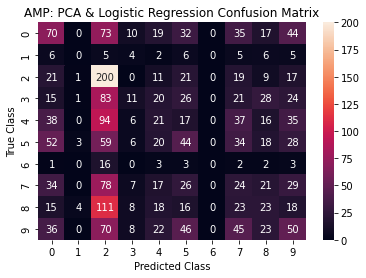
\includegraphics[width=0.45\linewidth]{cfm_lr_pca_amp.png}
    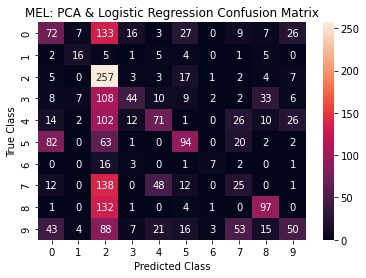
\includegraphics[width=0.45\linewidth]{cfm_lr_pca_mel.png}
\end{center}

\subsection{Random Forest Models}

\begin{table}[H]
\centering
\caption{Results of random forest models trained on AMP and MEL respectively with tuned hyperparameters (see section 2.2 for further discussion on choice of hyperparameters)}
\begin{tabular}{|c|c|c|}
 \toprule
 Random Forest Model & AMP (\%) & MEL (\%)\\
 \midrule
 Overall Training Accuracy & 100.0 & 100.0 \\
 Overall Test Accuracy & 27.5 & 47.8 \\
 Class 0 Accuracy & 4 & 38\\
 Class 1 Accuracy & 0 & 32\\
 Class 2 Accuracy & 41 & 47\\
 Class 3 Accuracy & 33 & 49\\
 Class 4 Accuracy & 26 & 49\\
 Class 5 Accuracy & 41 & 48\\
 Class 6 Accuracy & 0 & 52\\
 Class 7 Accuracy & 26 & 47\\
 Class 8 Accuracy & 5 & 53\\
 Class 9 Accuracy & 17 & 53\\
 \bottomrule
\end{tabular}
\end{table}
\begin{center}
    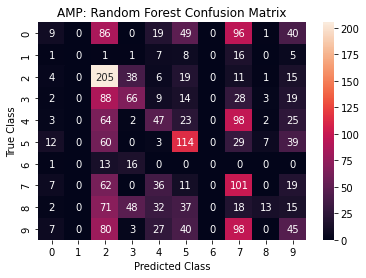
\includegraphics[width=0.45\linewidth]{cfm_rf_amp.png}
    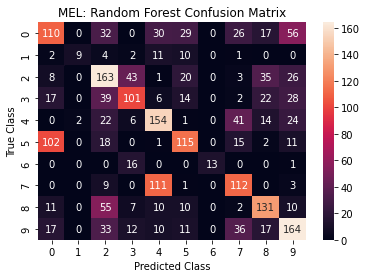
\includegraphics[width=0.45\linewidth]{cfm_rf_mel.png}
\end{center}

\newpage

\subsection{Hyperparameter Tuning and Validation}

\subsubsection{PCA \& Logistic Regression Models}
\begin{table}[H]
\centering
\caption{Tuning Regularization Strength \texttt{C} for AMP: PCA \& Logistic Regression Model}
\begin{tabular}{|c|c|c|c|}
 \toprule
 Parameter C & Mean Test & Std Dev  & Ranking\\
 \midrule
 0.25 & 0.171 & 0.0216 & 1\\
 0.5 & 0.170 & 0.0225 & 2\\
 1 & 0.167 & 0.0214 & 3\\
 1.5 & 0.167 & 0.0214 & 3\\
 2 & 0.167 & 0.0214 & 3\\
 \bottomrule
\end{tabular}
\end{table}

\begin{table}[H]
\centering
\caption{Tuning Regularization Strength \texttt{C} for MEL: PCA \& Logistic Regression Model}
\begin{tabular}{|c|c|c|c|}
 \toprule
 Parameter C & Mean Test & Std Dev  & Ranking\\
 \midrule
 0.25 & 0.329 & 0.0176 & 4\\
 0.5 & 0.329 & 0.0177 & 5\\
 1 & 0.329 & 0.0181 & 2\\
 1.5 & 0.329 & 0.0177 & 3\\
 2 & 0.330 & 0.0175 & 1\\
 \bottomrule
\end{tabular}
\end{table}

\subsubsection{Random Forest Models}
\begin{table}[H]
\centering
\caption{Tuning Depth \& Estimators for AMP: Random Forest Model (Top 5 pairs)}
\begin{tabular}{|c|c|c|c|c|}
 \toprule
 Depth & Estimators & Mean Test & Std Dev & Ranking\\
 \midrule
 32 & 500 & 0.239 & 0.027 & 1\\
 8 & 500 & 0.239 & 0.028 & 2\\
 16 & 500 & 0.239 & 0.021 & 3\\
 None & 500 & 0.238 & 0.033 & 4\\
 32 & 250 & 0.231 & 0.028 & 5\\
 \bottomrule
\end{tabular}
\end{table}

\begin{table}[H]
\centering
\caption{Tuning Depth \& Estimators for MEL: Random Forest Model (Top 5 pairs)}
\begin{tabular}{|c|c|c|c|c|}
 \toprule
 Depth & Estimators & Mean Test & Std Dev & Ranking\\
 \midrule
 32 & 500 & 0.549 & 0.041 & 1\\
 None & 500 & 0.547 & 0.045 & 2\\
 None & 250 & 0.544 & 0.047 & 3\\
 32 & 250 & 0.544 & 0.042 & 4\\
 16 & 500 & 0.541 & 0.040 & 5\\
 \bottomrule
\end{tabular}
\end{table}

\end{document}